% Fig. candidate for III-D: how the clock and the map predict and flag a deviation.
% One column (3.5 in = 252 pt). Build: pdflatex clock_and_map.tex
\documentclass[tikz,border=1pt]{standalone}
\usepackage[T1]{fontenc}
\usepackage{newtxtext,newtxmath}
\usetikzlibrary{arrows.meta,calc,decorations.markings}

\definecolor{ours}{HTML}{2A78D6}
\definecolor{oursbg}{HTML}{E8F1FC}
\definecolor{alarm}{HTML}{D03B3B}
\definecolor{ink}{HTML}{0B0B0B}
\definecolor{muted}{HTML}{52514E}
\definecolor{faint}{HTML}{BDBCB6}

\tikzset{
  font=\footnotesize,
  >={Stealth[length=3.4pt,width=2.8pt]},
  lab/.style={font=\scriptsize\itshape, text=muted, inner sep=1pt},
  panel/.style={font=\scriptsize\bfseries, anchor=north west, inner sep=0pt},
}

\begin{document}
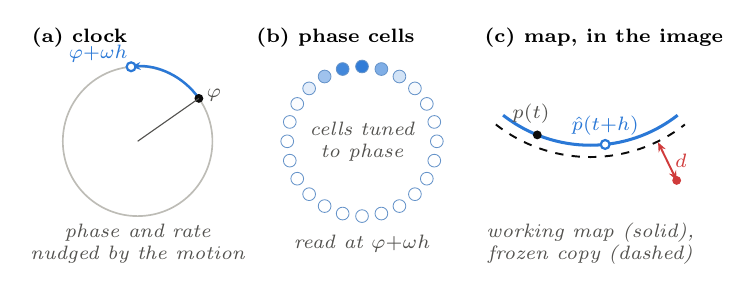
\begin{tikzpicture}

\def\R{0.95}          % clock / ring radius, cm
\def\ph{35}           % current phase, deg
\def\ah{95}           % phase advanced by omega*h, deg

% ---------------- (a) clock ----------------
\begin{scope}
  \node[panel] at (-1.35,1.45) {(a) clock};
  \draw[faint, line width=0.6pt] (0,0) circle (\R);
  \draw[->, ours, line width=0.9pt] (\ph:\R) arc[start angle=\ph, end angle=\ah, radius=\R];
  \fill[ink] (\ph:\R) circle (1.6pt);
  \draw[ours, fill=white, line width=0.8pt] (\ah:\R) circle (1.6pt);
  \node[lab, anchor=west] at (\ph:\R+0.07) {$\varphi$};
  \node[lab, anchor=south east, text=ours] at (\ah:\R+0.02) {$\varphi{+}\omega h$};
  \draw[muted, line width=0.4pt] (0,0) -- (\ph:\R);
  \node[lab, align=center] at (0,-1.3) {phase and rate\\nudged by the motion};
\end{scope}

% ---------------- (b) ring of phase cells ----------------
\begin{scope}[xshift=2.85cm]
  \node[panel] at (-1.35,1.45) {(b) phase cells};
  \foreach \a in {0,15,...,345} {
    % activity bump centred on the advanced phase
    \pgfmathsetmacro{\d}{min(abs(\a-\ah), 360-abs(\a-\ah))}
    \pgfmathsetmacro{\act}{100*exp(-(\d/28)^2)}
    \fill[ours!\act!white, draw=ours!60!faint, line width=0.3pt] (\a:\R) circle (2.3pt);
  }
  \node[lab, align=center] at (0,0) {cells tuned\\to phase};
  \node[lab, align=center] at (0,-1.3) {read at $\varphi{+}\omega h$};
\end{scope}

% ---------------- (c) map in the image ----------------
\begin{scope}[xshift=5.75cm]
  \node[panel] at (-1.35,1.45) {(c) map, in the image};
  % a pendulum-like arc about a pivot above; the frozen copy dashed, the working map solid
  \coordinate (pivot) at (0,1.75);
  \def\rf{1.95}\def\rw{1.8}
  \draw[ink, dashed, line width=0.7pt] ($(pivot)+(-128:\rf)$) arc[start angle=-128, end angle=-52, radius=\rf];
  \draw[ours, line width=1.1pt] ($(pivot)+(-128:\rw)$) arc[start angle=-128, end angle=-52, radius=\rw];
  \fill[ink] ($(pivot)+(-112:\rw)$) coordinate (now) circle (1.6pt);
  \node[lab, anchor=south] at ($(now)+(-0.08,0.1)$) {$p(t)$};
  \draw[ours, fill=white, line width=0.8pt] ($(pivot)+(-84:\rw)$) coordinate (next) circle (1.6pt);
  \node[lab, text=ours, anchor=south] at ($(next)+(0,0.07)$) {$\hat{p}(t{+}h)$};
  % an observation that has left the remembered path: the deviation distance d
  \coordinate (obs) at ($(pivot)+(-64:2.5)$);
  \draw[alarm, line width=0.7pt, <->, shorten >=0.3pt] (obs) -- ($(pivot)+(-64:\rf)$);
  \fill[alarm] (obs) circle (1.6pt);
  \node[lab, text=alarm, anchor=west] at ($(obs)!0.5!($(pivot)+(-64:\rf)$) + (0.06,0)$) {$d$};
  \node[lab, align=center] at (0,-1.3) {working map (solid),\\frozen copy (dashed)};
\end{scope}

\end{tikzpicture}
\end{document}
